\newpage
\fancyhf{}
\lhead{Dennis Hufnagel}
\rhead{Seite \thepage}
\section{Feuchtigkeitssensor}
\subsection{Warum ein Feuchtigkeitssensor?}
Um das automatische Pflanzenbewässerungssystem zu realisieren, standen uns zwei
verschiedene Herangehensweisen zur Verfügung. Einerseits hätte man die Bewässerung nur
mit einem zeitbasierten Algorithmus durchführen können. Andererseits bestand die
Möglichkeit, als Basis für die Bewässerung auf Feuchtigkeitsmessungen zurückzugreifen.

\subsubsection{Nachteile/Vorteile einer rein zeitbasierten Bewässerung}
Ein großer Nachteil dieses Ansatzes ist, dass die Bewässerungsroutine zeitlich festgelegt ist.
So ist es praktisch unmöglich, auf sich verändernde Einflüsse in der Umgebung der Pflanze zu
reagieren. Eine Veränderung der Sonneinstrahlung, des Wetters und somit der
Luftfeuchtigkeit oder der Temperatur beeinflussen, wie schnell die Erde im Blumentopf
austrocknet. Während einer regnerischen und gleichzeitig kalten Jahreszeit, könnte die
Pflanze aufgrund der festen Bewässerungsroutine ertränkt werden, da die Erde während
eines Bewässerungsintervalls nicht stark genug trocknet. Dasselbe gilt natürlich auch
andersrum, dass die Pflanze während eines Intervalls zu stark austrocknet. Außerdem muss
für jede einzelne Pflanze ein individuelles Profil erstellt werden, da Pflanze unterschiedlich
viel Wasser benötigen. Somit besteht die Möglichkeit, dass die Pflanzen zu früh eingehen, da
nicht immer für optimale Bedingungen gesorgt werden konnte. Eine Option, dieses Problem
ohne Feuchtigkeitssensor zu beheben, wäre die Verwendung von Temperatursensoren und
die Miteinbeziehung von den lokalen Wetterdaten. So könnte man mit einer Kalkulation die
Zustände in der Erde und den Grad der Austrocknung approximieren. Dieses Verfahren ist
allerdings extrem umständlich und würde so den Rahmen dieser Projektarbeit sprengen.
Der Vorteil dieses Verfahrens ist seine Einfachheit bei der Anlegung der Routine. Zwar muss
für jede Pflanze eine eigene Erstellt werden, jedoch müssen keine Berechnungen oder
Messungen vorgenommen werden, um Sensoren zu kalibrieren und deren Daten mit dem
Feuchtigkeitsgrad der Erde zu korrelieren. Es muss lediglich die Routine programmiert
werden, damit das System einwandfrei funktioniert.

\subsubsection{Nachteile/Vorteile einer sensorbasierten Bewässerung}
Der größte Vorteil, der ein Feuchtigkeitssensor mit sich bringt, ist, dass der Zustand der Erde
gemessen werden kann. Somit können die äußeren Einflüsse ignoriert werden, da wir deren
Ergebnisse, die unterschiedlich schnell austrocknende Erde, messen können. Somit ist dieses
Verfahren flexibler und universeller anwendbar. Für unterschiedliche Pflanze müssen jetzt
keine individuellen Routinen programmiert werden, da Pflanzen, die z.B. weniger Wasser
benötigen, die Erde einfach langsamer austrocknen. So müssen nur die Daten ausgelesen
werden und daraufhin kann dann entschieden werden, ob gewässert werden muss oder
nicht.
Ein Nachteil dieser Technik ist die Notwendigkeit, Sensoren zu entwickeln und immer für die
unterschiedlichen Erden zu kalibrieren. Dies ist wichtig, damit der Sensor eine trockene Erde
auch als solche ausliest. Letztendlich ist dieser Ansatz jedoch der Effizientere.

\subsection{Entwurf des Feuchtigkeitssensors}
\subsubsection{Theorie des Sensors} \label{sensortheorie}
Zuallererst musste entschieden werden, ob fertige Sensoren gekauft werden, oder der
Sensor selber entwickelt wird. Da wir zu viert an dieser Projektarbeit gearbeitet haben,
konnten die Sensoren selber entwickelt werden, da genug Ressourcen vorhanden waren.
Nachdem dies geklärt war, musste eine Entscheidung zwischen der kapazitiven und der
resistiven Messmethode getroffen werden. Aufgrund der Probleme durch die mögliche
Elektrolyse in der Erde, wurde sich für die kapazitive Messmethode entschieden.
Die Formel um die Größe eines Kondensators zu bestimmen, lautet:
\begin{center}
    $C = \varepsilon _R * \varepsilon _0 * \frac{A}{d}$ (1)
\end{center}
Wobei $A$ der Fläche der Kondensatorplatten, $d$ dem Abstand zwischen den Platten, $\varepsilon _0$ der
elektrischen Feldkonstante und $\varepsilon _R$ der Permittivitätszahl entspricht. Das Prinzip der
kapazitiven Messmethode beruht darauf, dass sich mit einer Änderung der Feuchtigkeit auch
die Permittivitätszahl verändert. Da $\varepsilon _0$ eine Konstante ist und der geometrische Aufbau des
Sensors und somit des Kondensators sich nicht verändert, bleiben $A$ und $d$ auch konstant.
Somit ist die Größenveränderung des Kondensators ausschließlich von der sich ändernden
Permittivitätszahl abhängig.

\subsubsection{Schaltplan/Funktion des Sensors}
Nun musste die Schaltung für solch einen Sensor entwickelt werden. Dazu wurde im Internet
recherchiert und Konkurrenzprodukte analysiert. Letztendlich wurde sich dafür entschieden,
einen Schmitt-Trigger mit Hysterese zu verwenden. Die Hysterese dient dazu, den Schmitt-Trigger
weniger anfällig gegen Störungen zu machen. Hiermit lässt sich ein recht einfacher,
jedoch akkurater Sensor bauen.
\begin{figure}[ht]
    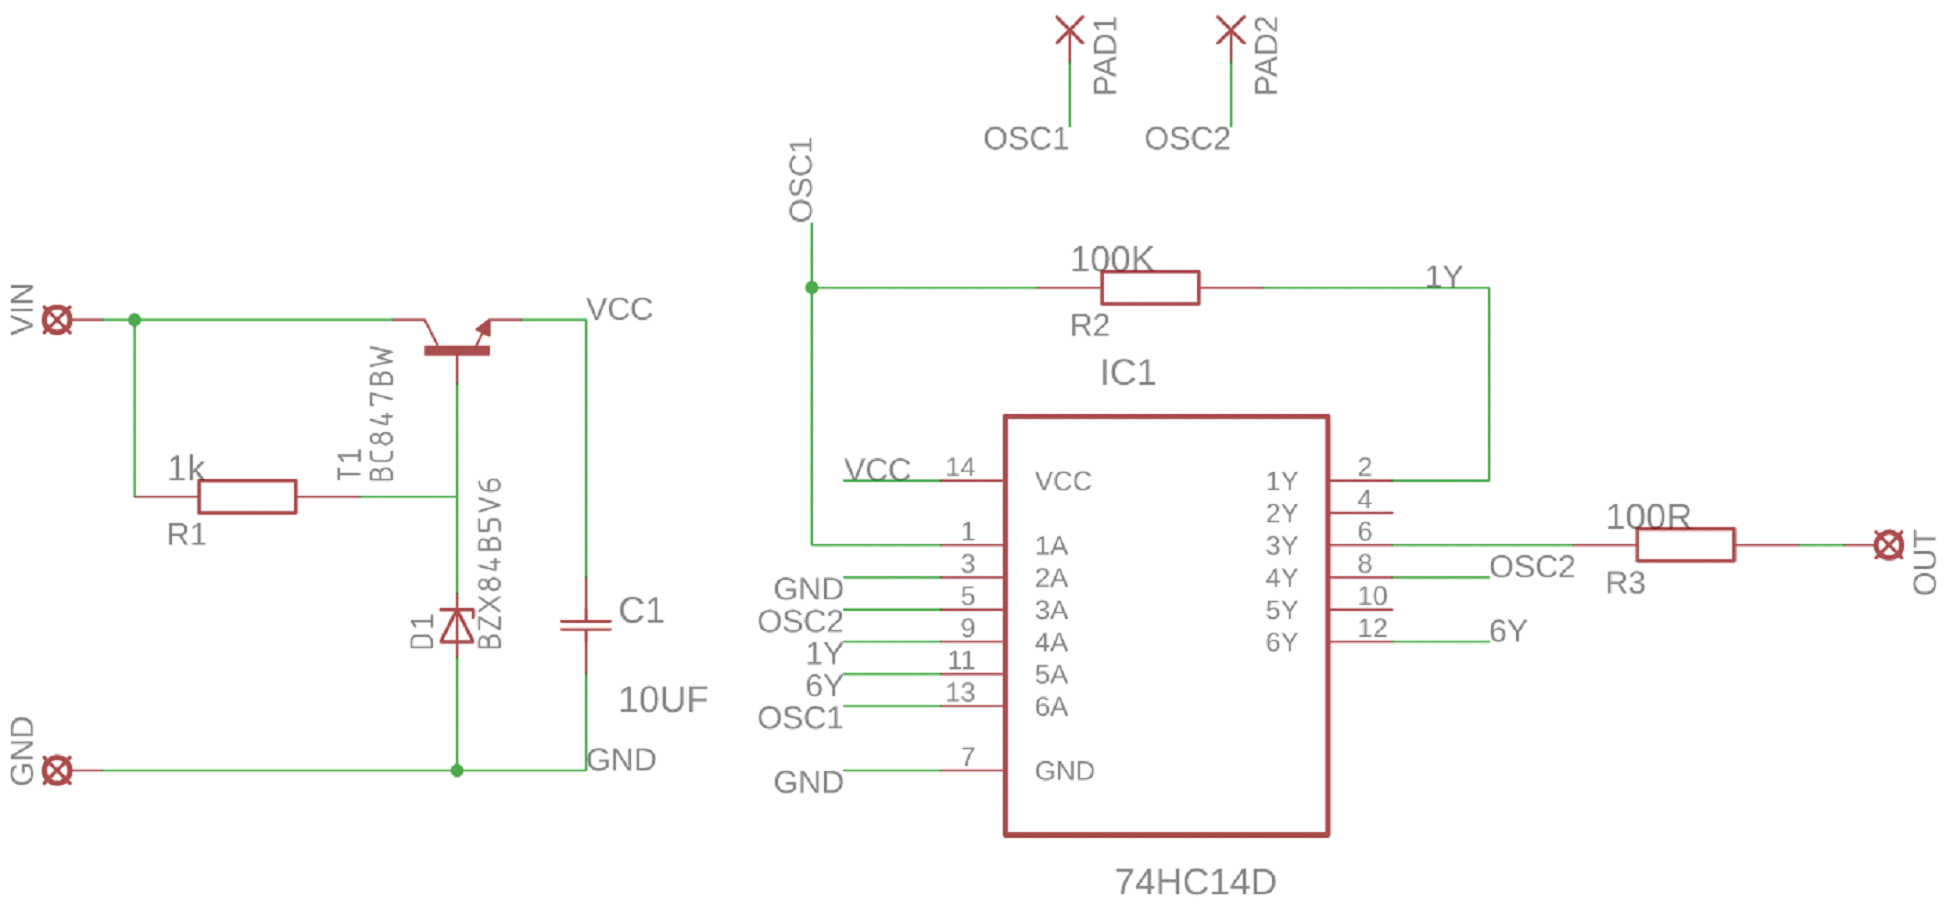
\includegraphics[width=\textwidth]{dennis/schaltplan}
    \caption{Schaltplan des Feuchtigkeissensors}
\end{figure}

Der $IC1$ besitzt bis zu sechs invertierende Schmitt-Trigger, welche jeweils von ihrem Eingang
$A$ bis zum Ausgang $Y$ verbaut sind. Versorgt wird er mit einer Gleichspannung von $5V$. Diese
wird von dem linken Teil der Schaltung erzeugt. Diese kleine Konstantan-Spannungsquelle
wurde eingefügt, da wir zu Beginn noch nicht wussten, mit welcher Spannung wir den Sensor
versorgen können. Der Schmitt-Trigger, der wichtig für unsere Schaltung ist, ist an seinem
Eingang 1A mit einer Kondensatorplatte OSC1 verbunden. Die Hysterese ist über den $100k\Omega$
Widerstand mit dem Ausgang $1Y$ verbunden. Die zweite Kondensatorplatte ist an dem
Schmitt-Trigger Eingang $3A$ angeschlossen. Der Ausgang $3Y$ ist noch mit einem $100\Omega$
Widerstand belastet, damit ein etwas höherer Strom durch die Leitungen fließt. Die anderen
Anschlüsse am I$C1$ als die oben genannten, dienen nur dem Zweck, das routen der
Leiterbahnen zu vereinfachen. Sie haben keinen Einfluss auf die Funktionalität der Schaltung.
Da der Schmitt-Trigger invertierend ist, lädt er, solange die Schaltschwelle noch nicht
erreicht ist, den Kondensator über den Widerstand auf. Diese erste Kondensatorplatte $OSC1$
lädt somit die zweite Platte $OSC2$ auf. Erreicht die zweite Kondensatorplatte somit die
Schwellenspannung, wechselt der Schmitt-Trigger an seinem Ausgang $3Y$ von 1 auf 0 und
entlädt die Kondensatorplatte $OSC2$ dabei. Nun beginnt dasselbe Prinzip wieder von vorne.
$OSC2$ wird wieder aufgeladen und der Schmitt-Trigger wechselt beim Erreichen seiner
Schwellenspannung wieder von 1 auf 0. Da die Zeit, die benötigt wird um den Kondensator
aufzuladen, abhängig von dessen Größe ist, haben wir eine variable Frequenz, die von der
Größe des Kondensators abhängig ist. Da wir unter Kapitel \ref{sensortheorie} gelernt haben
, dass die Größe des Kondensators nur von der Permittivitätszahl abhängig ist, bedeutet das, dass die
Frequenz, mit der unser Schmitt-Trigger schaltet, von der Permittivitätszahl und somit von
dem Feuchtigkeitsgrad der Erde abhängig ist. Je trockener die Erde, desto kleiner wird die
Permittivitätszahl und somit der Kondensator. Somit liefert der Sensor bei trockener Erde
eine höhere Frequenz als bei nasser, da der Kondensator schneller aufgeladen wird. Der
Verlauf der Frequenz in Abhängigkeit von dem Feuchtigkeitsgrad der Erde verläuft linear.
Somit haben wir am $OUT$ Ausgang unsere Schaltung ein $5V$ Signal mit variierender Frequenz
anliegen, welches wir mit dem Arduino UNO auslesen können.
Das Erstellen des Platinenlayouts des Sensors wird im Kapitel \ref{sensorlayout} beschrieben.

\subsubsection{Messergebnisse des Sensors}
Nachdem das Layout des Sensors fertiggestellt wurde (Kap. \ref{sensorlayout}), konnte die Platine mit der
Ätzmaschine der Hochschule geätzt werden. Danach konnten auf jedem Sensor die Bauteile
aufgebracht und festgelötet werden. Damit sichergestellt werden kann, dass jeder Sensor
problemlos funktioniert und alle Lötstellen korrekt angebracht wurden, muss jeder Sensor
einem Funktionstest unterzogen werden. Dazu wird jeder einzelne Sensoren an $+5V$ und das
$OUT$-Signal an ein Oszilloskop angeschlossen. Der Sensor wurde dann zuerst an der Luft
getestet, um seine korrekte Funktionsweise zu überprüfen. War dies Erfolgreich, wurde der
Sensor mit dem Schutzlack Plastik 70 eingesprüht, um die Platine vor Korrosion zu schützen.
Danach wurde der Sensor in einen kleinen Behälter mit Erde gesteckt. Diese war kaum mit
Wasser angesetzt, um den Sensor in trockenen Verhältnissen zu testen.
\begin{figure}[ht]
    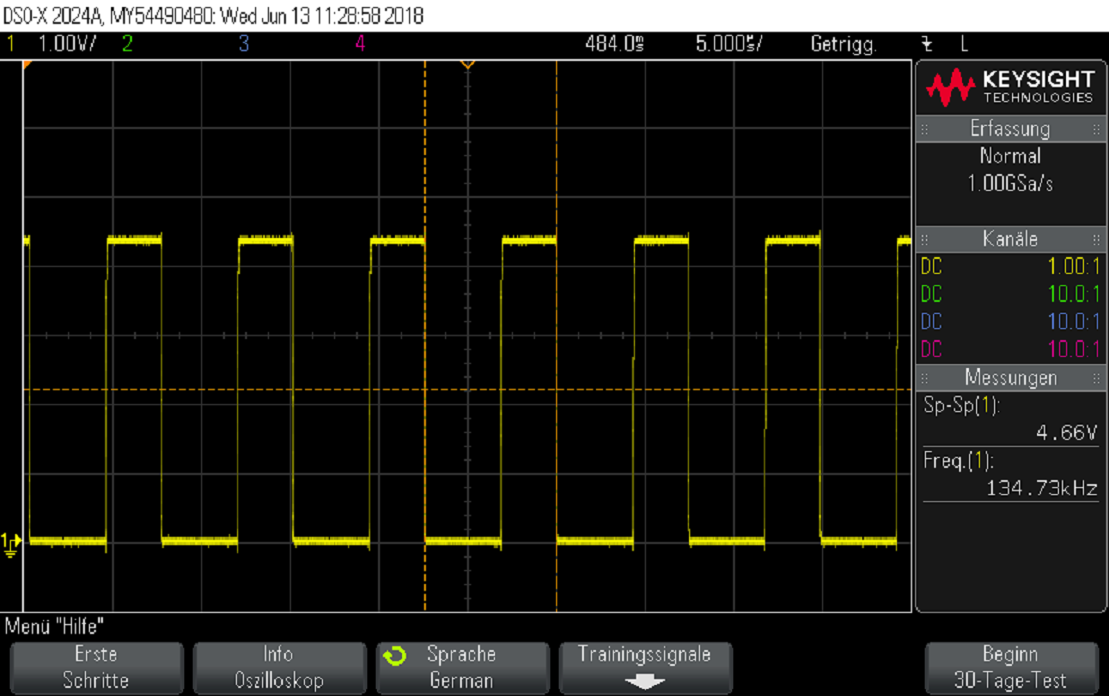
\includegraphics[width=\textwidth]{dennis/trocken}
    \caption{Auslesen des Sensors bei trockener Erde}
\end{figure}
Dann wurde etwas Wasser in die Erde gegossen und, wie zu erwartend, eine Verringerung der
Frequenz festgestellt.
Somit konnte die korrekte Funktionsweise jedes Sensors bewiesen werden.
\begin{figure}[ht]
    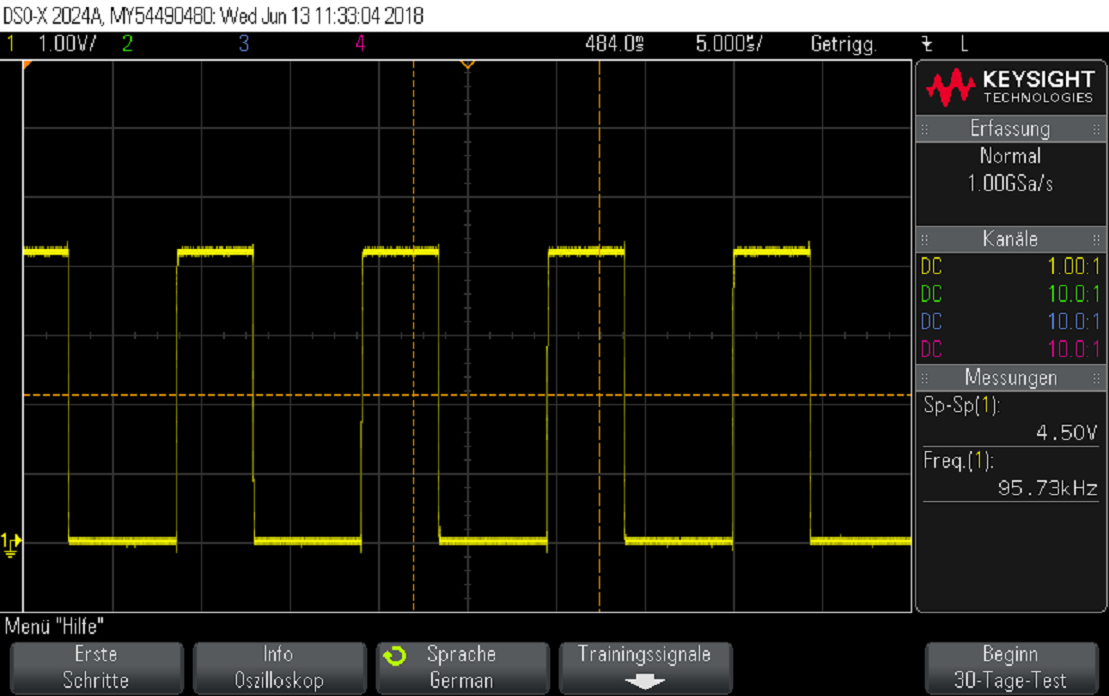
\includegraphics[width=\textwidth]{dennis/feucht}
    \caption{Auslesen des Sensors bei feuchter Erde}
\end{figure}

\section{Erstellen der Platinenlayouts}
\subsection{Layout des Feuchtigkeitssensors} \label{sensorlayout}
Bevor damit begonnen werden konnte, den Sensor in Eagle zu routen, musste festgelegt
werden, inwiefern der Sensor aufgebaut wird. Der Aufbau eines normalen Kondensators
besteht aus zwei gegenüberliegenden Platten (Abbildung \ref{fig:kond1}). Dieser Aufbau würde sich
allerdings als relativ umständlich erweisen, da man somit den Sensor in drei einzelne
Platinen aufteilen müsste. Je zwei für die zwei Kondensatorenplatte und die dritte Platine für
die Elektronik. Diese Platinen müsste man noch über Winkel dann miteinander fixieren,
damit der Abstand der Kondensatorplatten zueinander auch konstant bleibt. Da dieser
Aufbau somit zu umständlich war, wurde nach Alternativen gesucht. Das Ergebnis ist, dass
die beiden Kondensatorplatten jetzt nebeneinander, anstatt übereinander, angelegt werden.
Dies wird in Abbildung \ref{fig:kond2} verdeutlicht.
\begin{figure}[ht]
    \centering
    \begin{minipage}{0.45\textwidth}
        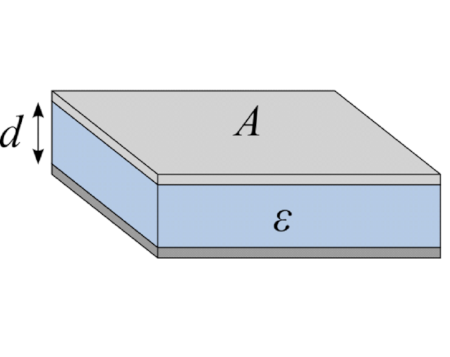
\includegraphics[width=0.9\textwidth]{dennis/kond1}
        \caption{Kondensatorplatten übereinander}
        \label{fig:kond1}
    \end{minipage}
    \begin{minipage}{0.45\textwidth}
        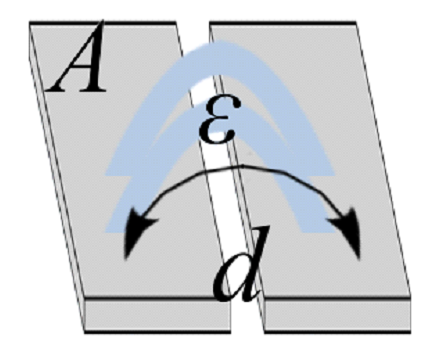
\includegraphics[width=0.9\textwidth]{dennis/kond2}
        \caption{Kondensatorplatten nebeneinander}
        \label{fig:kond2}
    \end{minipage}
\end{figure}
Ein Problem dieses Ansatzes ist allerdings, dass sich die Geometrie ändert und somit die
Formel (1) nicht mehr stimmt. Da allerdings, wie unter Kapitel \ref{sensortheorie} beschrieben, die
Geometrie konstant bleibt, ist die Änderung der Kondensatorgröße weiterhin nur von der
Permittivitätszahl abhängig. Die veränderte Geometrie spielt somit für die Funktion der
Schaltung keine Rolle. Nun konnte mit dem Anlegen des Platinenlayouts begonnen werden.
\begin{figure}[h]
    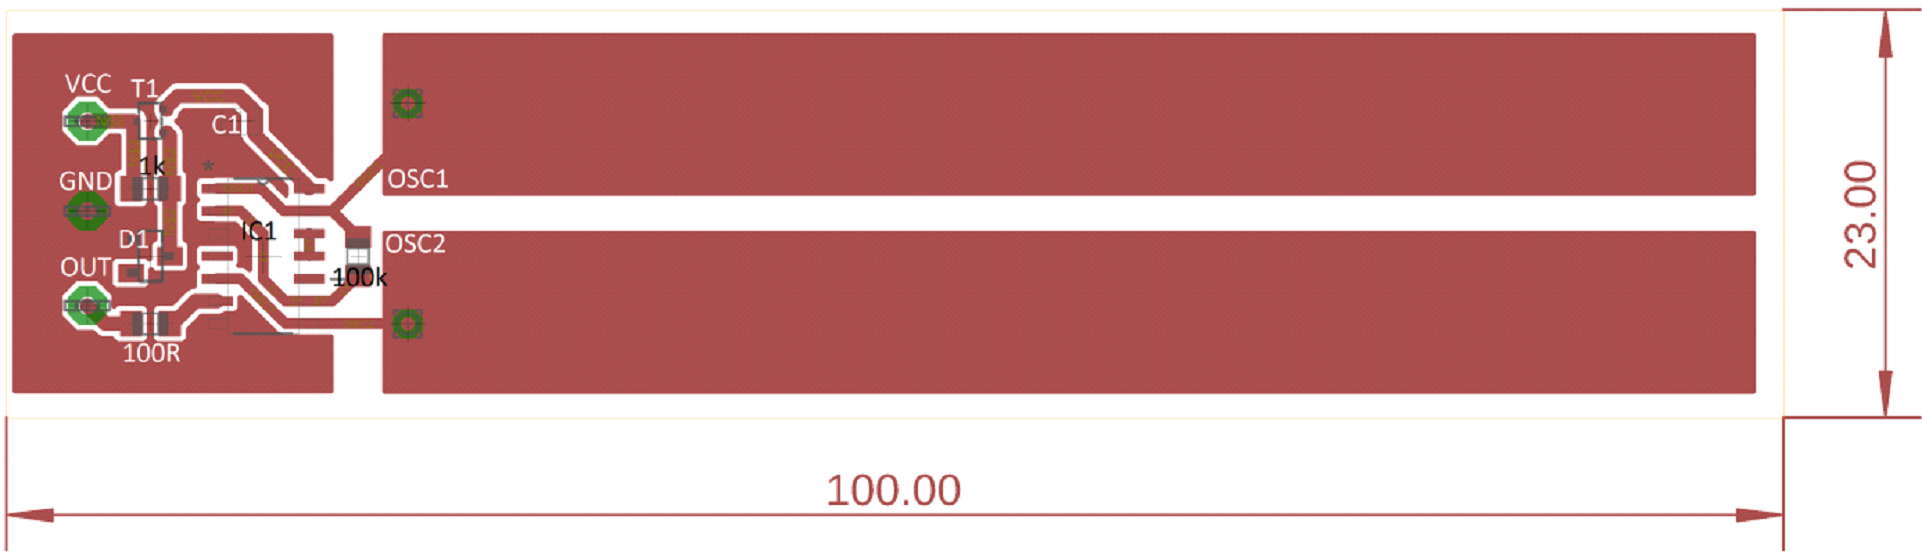
\includegraphics[width=\textwidth]{dennis/layout2}
    \caption{Layout des Feuchtigkeissensors}
\end{figure}
Die elektronischen Bauteile wurden auf der linken Seite angeordnet. Während die beiden
großen Kupferpolygone auf der rechten Seite die Kondensatorplatten repräsentieren. Somit
kann der Sensor in die Erde gesteckt werden, ohne dass die Bauteile mit der Erde in Kontakt
treten müssen. Generell wurden die Bauteile so kompakt wie möglich angeordnet, damit die
Platine am Ende nicht zu groß wird. Der Sensor muss natürlich in jeden Blumentopf passen.
Die drei Anschlüsse der Platine ($VCC$, $GND$, $OUT$) wurden für eine gute Erreichbarkeit, ganz
am Rand angebracht. Dadurch müssen auch die Kabel nicht durch die Erde geführt werden.
Für einen besseren Anschluss der $GND$-Pins der Bauteile, wurde ein $GND$-Polygon um die
Bauteile herum angebracht. Dadurch wird der Stromfluss des $GND$-Potentials verbessert. Die
restlichen Verbindungen wurden dann, je nach Möglichkeit, mit einer möglichst breiten
Leiterbahn verbunden. Eine breitere Leiterbahn verbessert den Stromfluss.

\subsection{Layout der Leistungsschaltungsplatine}
\begin{figure}[h]
    \centering
    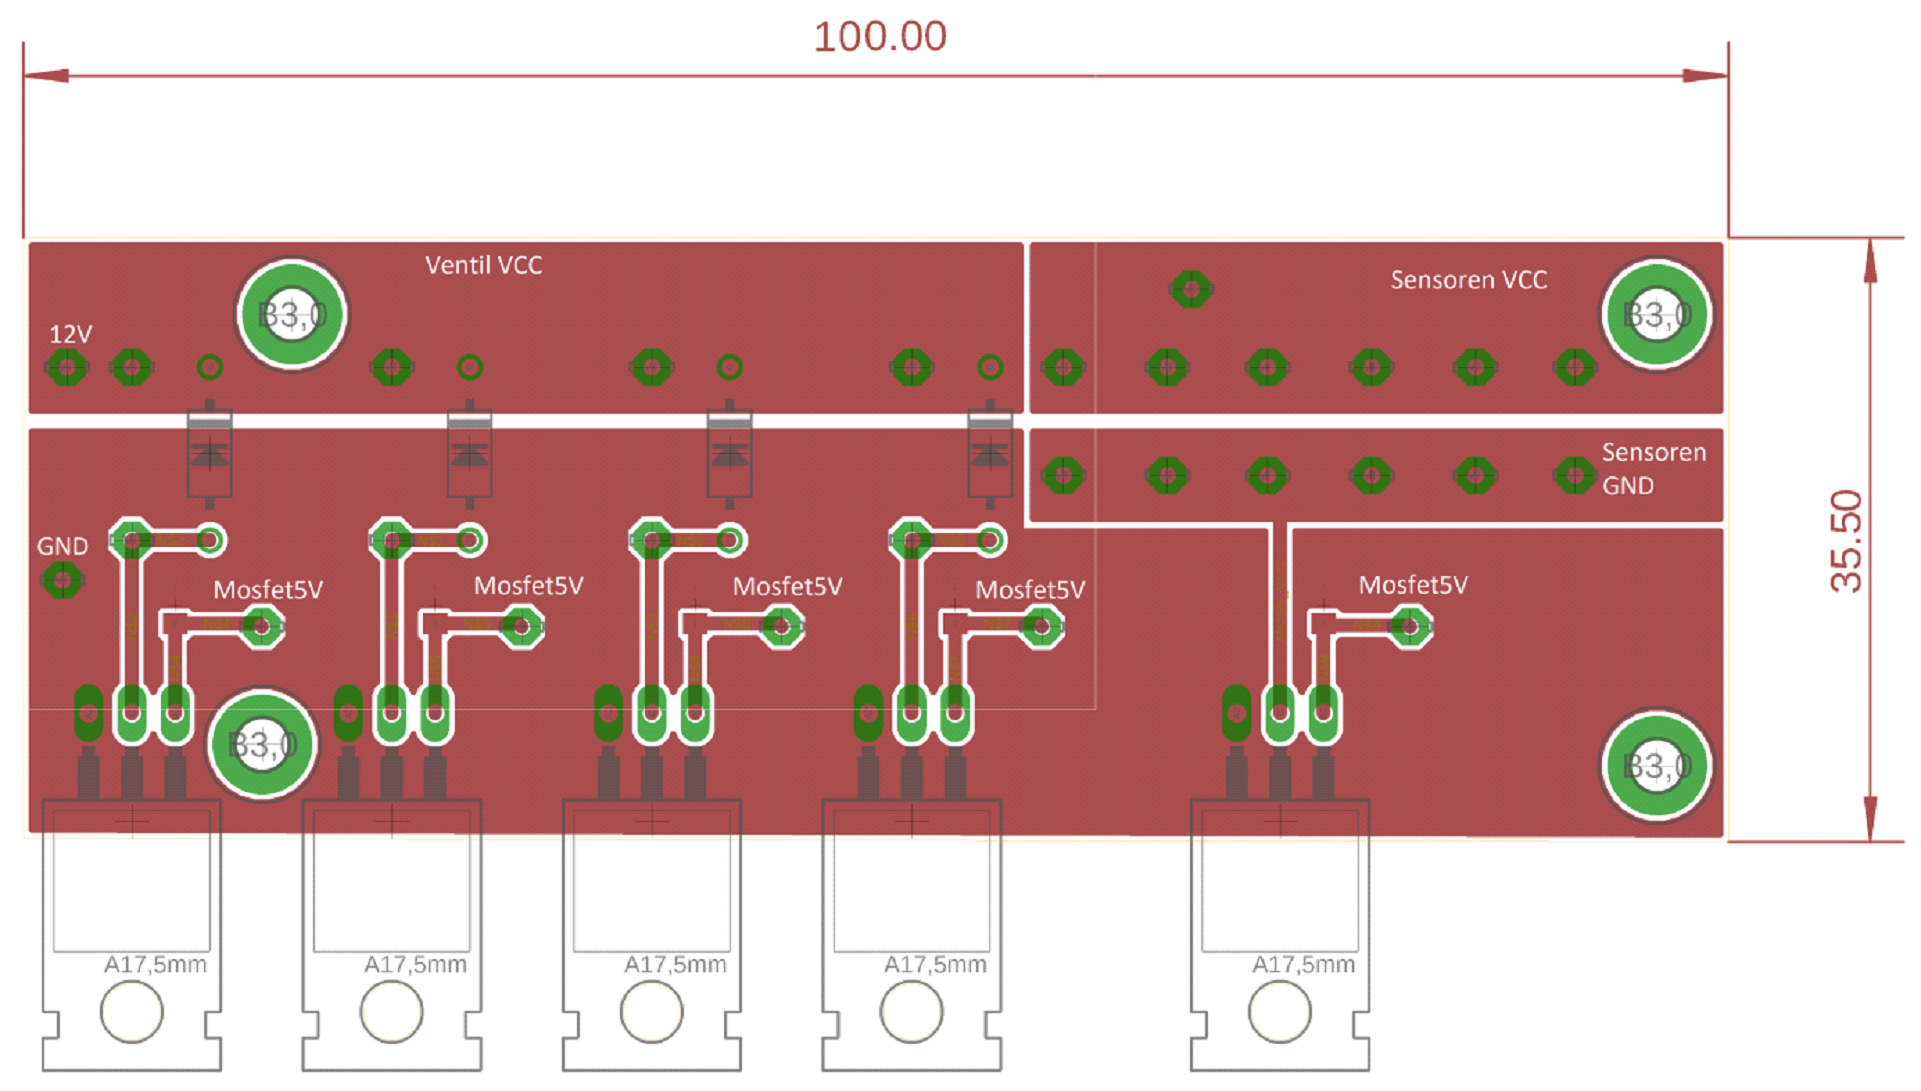
\includegraphics[width=\textwidth]{dennis/layout1}
    \caption{Layout der Leistungsschaltungsplatine}
\end{figure}

Die Ventile, die wir verwenden, benötigen $12V$ Versorgungsspannung und bis zu $300mA$
Strom. Dies kann der Arduino selbstverständlich nicht leisten. Deswegen musste eine
weitere Platine entworfen werden, die die Ansteuerung und Versorgung der Ventile, der
Pumpe und auch die Versorgung der Sensoren übernimmt. Der Entwurf der Schaltung und
die Entwicklung des Schaltplans hat mein Kollege Silas Leidel übernommen. Von mir wurde
dann noch das Layout angefertigt, da ich bereits Erfahrung damit hatte. Zur Steuerung der
Ventile, Sensoren und Pumpe wurde an jeden Anschluss ein MOSFET hinzugefügt. Die Pfade
für die Pumpe und die Ventile besitzen auch noch eine dazu parallele Rücklaufdiode. Die VCC
Anschlüsse der Ventile und Pumpen werden im linken, oberen $12V$ Polygon
angeschlossen. Ihr $GND$ Anschluss wird dann links, neben den Dioden VIA verlötet. Am
unteren Ende der Platine sitzt der MOSFET, der wiederum von dem Arduino über den
Mosfet $5V$ Anschluss gesteuert wird. Diese Anordnung existiert insgesamt viermal, dreimal
für die drei Ventile und einmal für die Pumpe. Da die Sensoren mit $5V$ versorgt werden,
musste für sie ein extra Polygon zur Stromversorgung angelegt werden. Versorgt wird dieses
Potential von der unter Kapitel \ref{stromlayout} vorgestellten Platine. Es wurde entschieden,
nur einen MOSFET für alle Sensoren zu verwenden, da sonst die Platine, wegen der
zusätzlichen MOSFET, zu groß geworden wäre. Um den Stromfluss zu verbessern, wurden
wieder alle Spannungspotentiale als Polygon realisiert. Am Ende wurden noch vier M3
Befestigungslöcher hinzugefügt, damit die Platine einfacher an einem Gehäuse befestigt
werden kann.

\subsection{Layout des Stromverteilers} \label{stromlayout}
\begin{figure}[h]
    \centering
    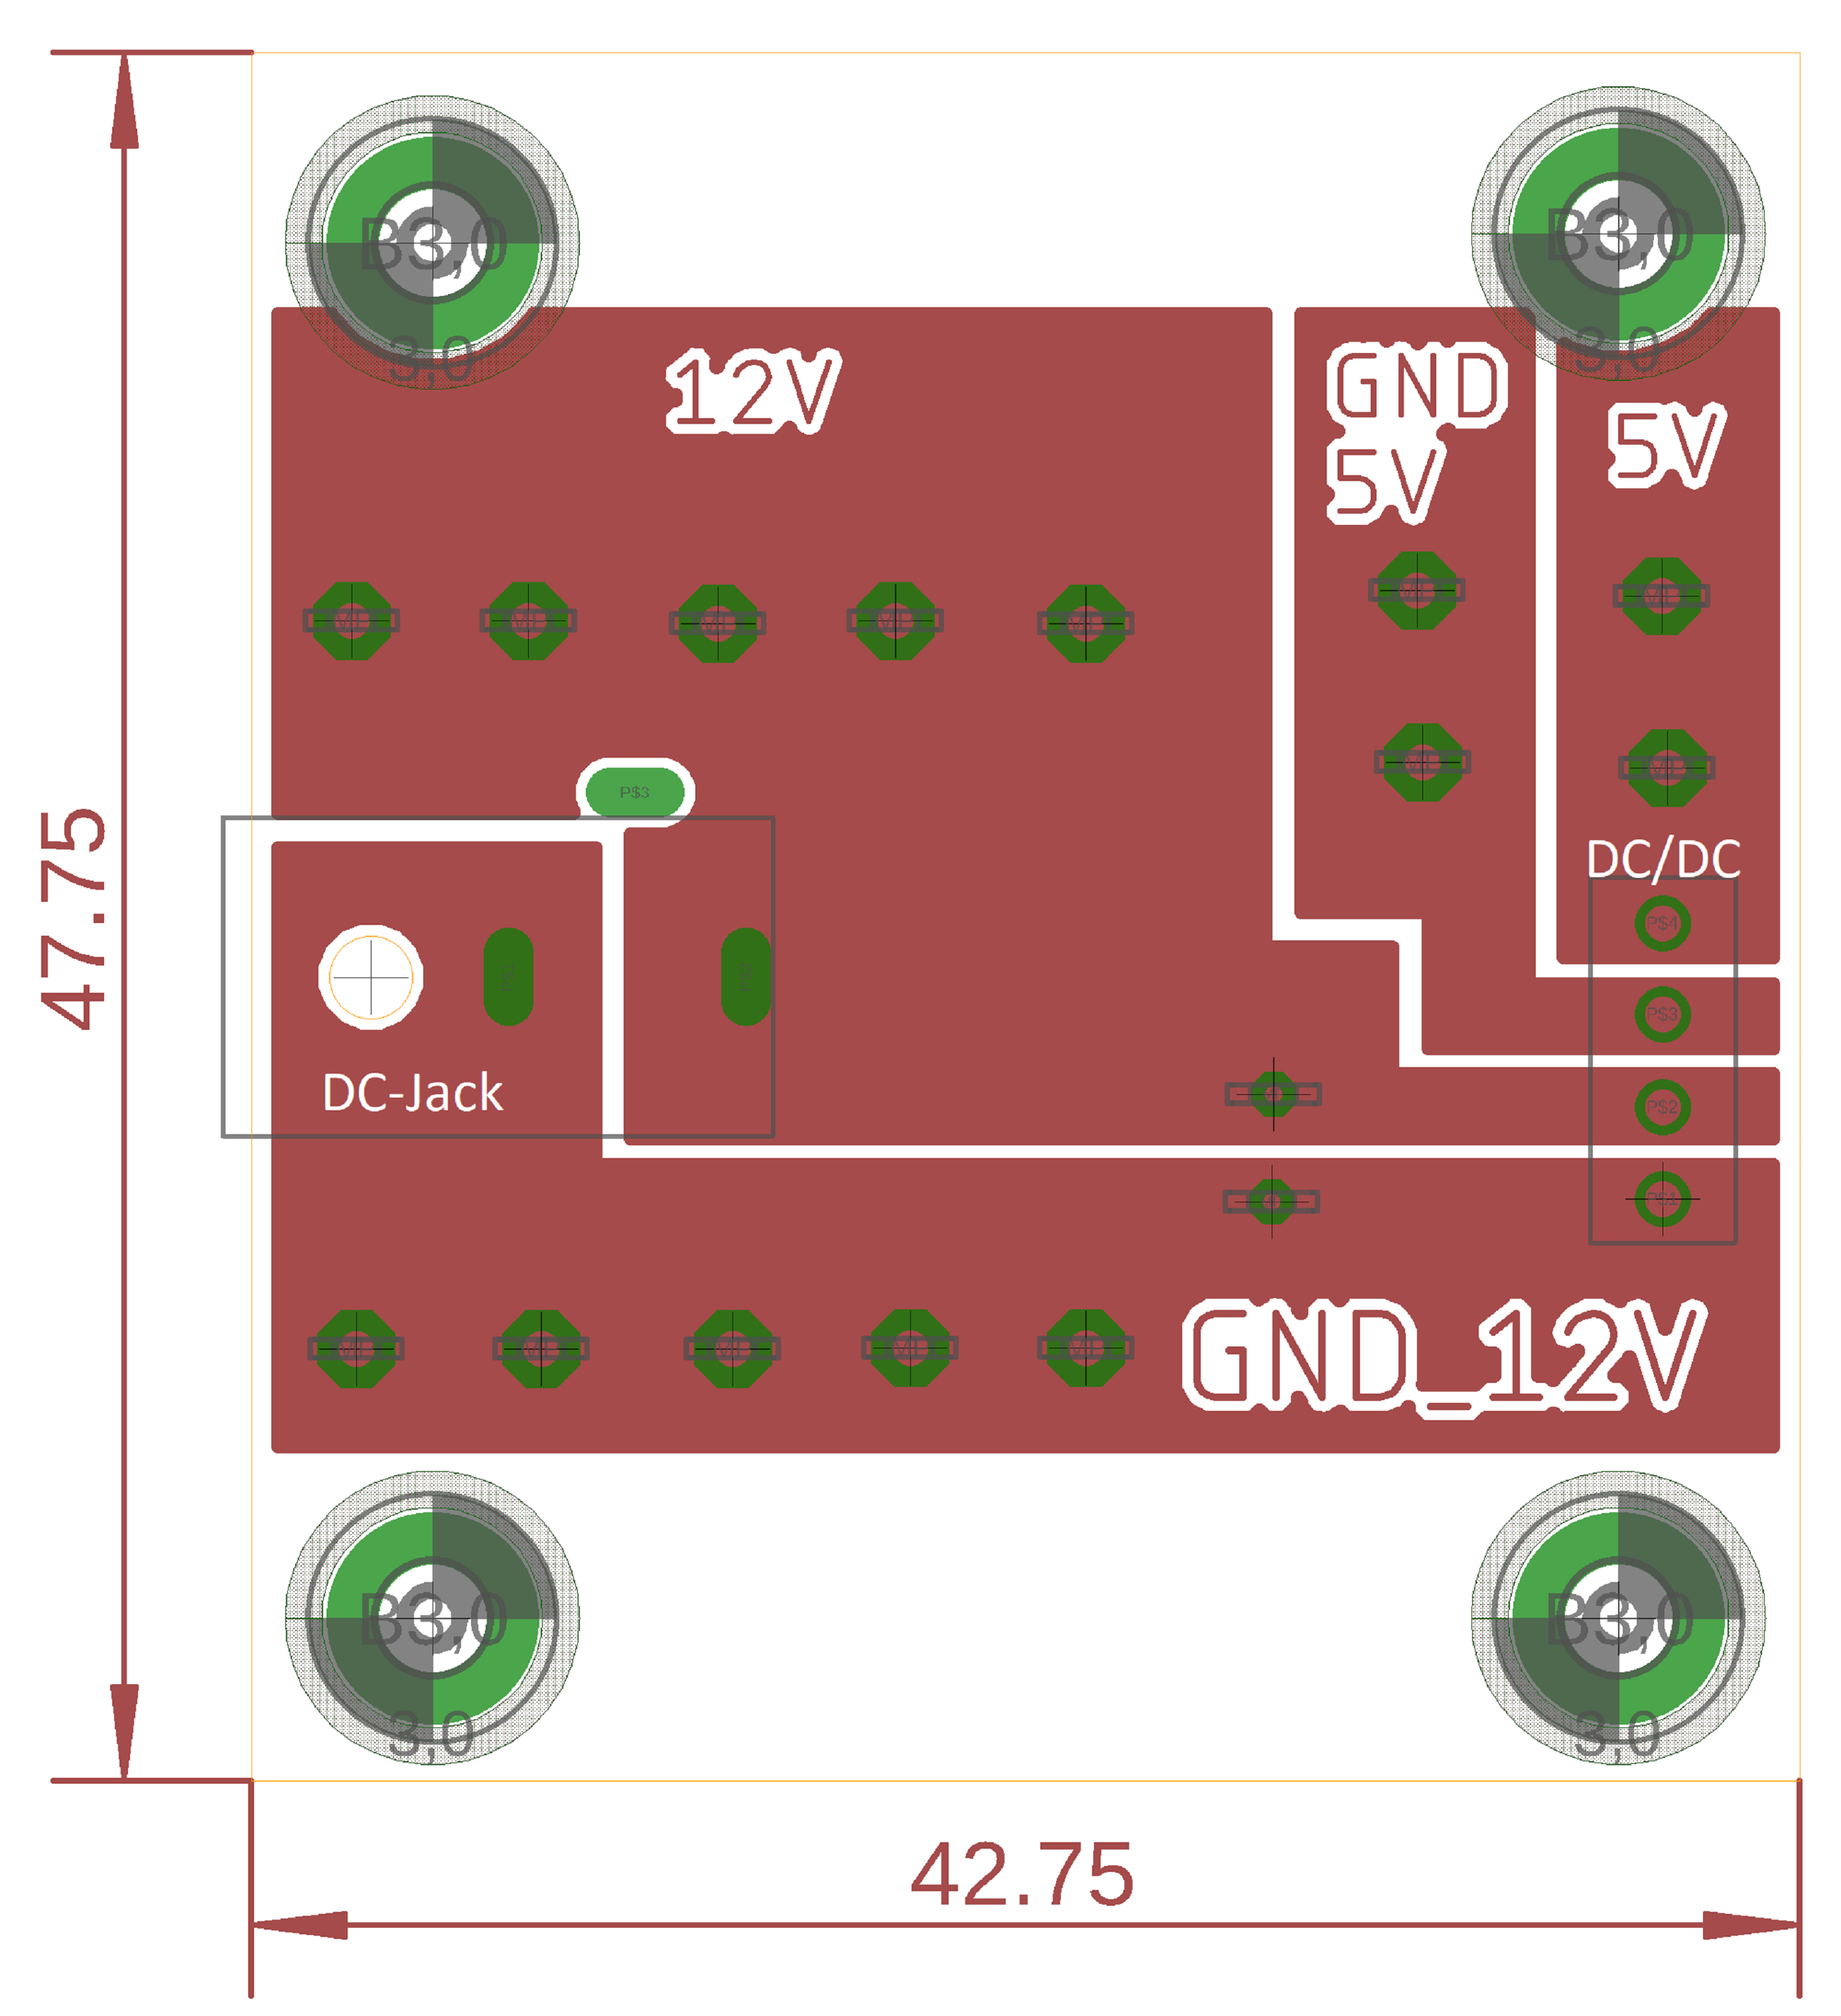
\includegraphics[width=0.5\textwidth]{dennis/layout}
    \caption{Layout der Stromverteilers}
\end{figure}
Diese Platine dient als Stromverteiler bzw. Stromwandler für unsere Elektronik. Die Sensoren
benötigen $5V$ Versorgungsspannung, während der Arduino, die Ventile und die Pumpe $12V$
brauchen. Das verwendete, externe Netzteil kann allerdings nur $12V$ liefern. Damit wir diese
$12V$ einerseits auf die verschiedenen Platinen und Bauteile verteilen können und
andererseits auf $5V$ umwandeln können, wurde diese Platine entworfen. Die Schaltung
stammt wieder von meinem Kollegen Silas Leidel. Der DC-Jack ist der Anschlussstecker an
das externe Netzteil, dass die 230V Wechsel- auf $12V$ Gleichspannung transformiert. Diese
$12V$ werden dann mit dem DC/DC Konverter auf $5V$ heruntertransformiert. Diese $5V$ dienen
dann als Versorgungsspannung für die Sensoren. Die verschiedenen Spannungspotentiale
sind auch hier wieder als Polygone ausgeführt. Letztendlich wurden der Platine noch vier M3
Bohrlöcher hinzugefügt, um ihre Befestigung am Gehäuse zu vereinfachen. Das Verlöten des
DC-Jack erwies sich jedoch in der Praxis als schwierig. Hierfür wäre es einfacher gewesen,
Polygone auf der Vorder- und Rückseite zu verwenden und diese mittels VIAs zu verbinden.